\documentclass[11pt,aps,a4paper,eqsecnum,amsmath,amssymb,longbibliography,notitlepage,nofootinbib]{revtex4-1}
\usepackage{amsthm,amssymb}
\usepackage{xcolor}
\usepackage{tikz}
\usetikzlibrary{decorations.markings}

\begin{document}

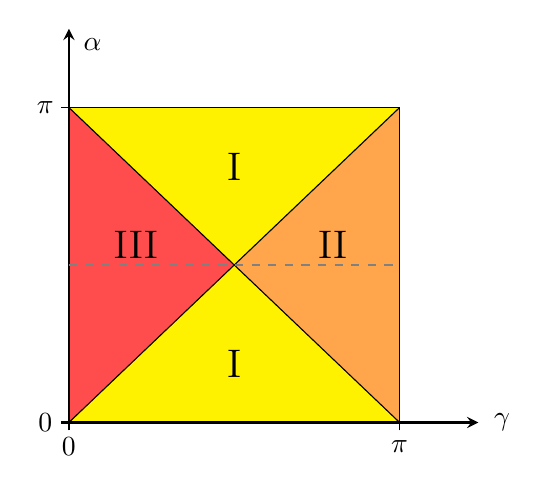
\begin{tikzpicture}

\path[fill =green, opacity = 1] (0,0) -- (4.2,0) -- (2.1,2) -- cycle;
\path[fill =yellow, opacity = 1] (0,0) -- (4.2,0) -- (2.1,2) -- cycle;
\path[fill = green, opacity = 1] (0,4) -- (4.2,4) -- (2.1,2) -- cycle;
\path[fill = yellow, opacity = 1] (0,4) -- (4.2,4) -- (2.1,2) -- cycle;
\path[fill = orange, opacity = 0.7] (4.2,0) -- (2.1,2) -- (4.2,4) -- cycle;
\path[fill = red, opacity = 0.7] (0,0) -- (2.1,2) -- (0,4) -- cycle;
\draw[-stealth,thick] (-0.1,0) -> (5.2,0); 
\draw[-stealth,thick] (0,-0.1) -> (0,5); 
\draw (4.2,-0.1) -- (4.2,4);
\draw (-0.1,4) -- (4.2,4);
\draw (0,0) -- (4.2,4);
\draw (0,4) -- (4.2,0);
\draw[dashed,gray] (0,2) -- (4.2,2);
\node at (-0.3,0) {$0$};
\node at (-0.3,4) {$\pi$};
\node at (0,-0.3) {$0$};
\node at (4.2,-0.3) {$\pi$};
\node at (3.35,2.25) {\Large II};
\node at (0.85,2.25) {\Large III};
\node at (2.1,0.75) {\Large I};
\node at (2.1,3.25) {\Large I};
\node at (5.5,0) {$\gamma$};
\node at (0.3,4.8) {$\alpha$};
\end{tikzpicture}

\end{document}